\section{Results}

In this section the Plastic Bistable Recurrent Cell is compared to the nBRC and Plastic GRU to determine its ability to memorize high-dimensional inputs for long periods of time. Plotted below are the losses of each of the Plastic GRU, nBRC and PBRC models over the course of training with an input dimension of 32 and a hidden state dimension of 64. All three models were able to solve the task in the number of iterations allotted, however the PBRC was able to solve it using far less data than the other two models.

\begin{figure}[h]
	\centering
	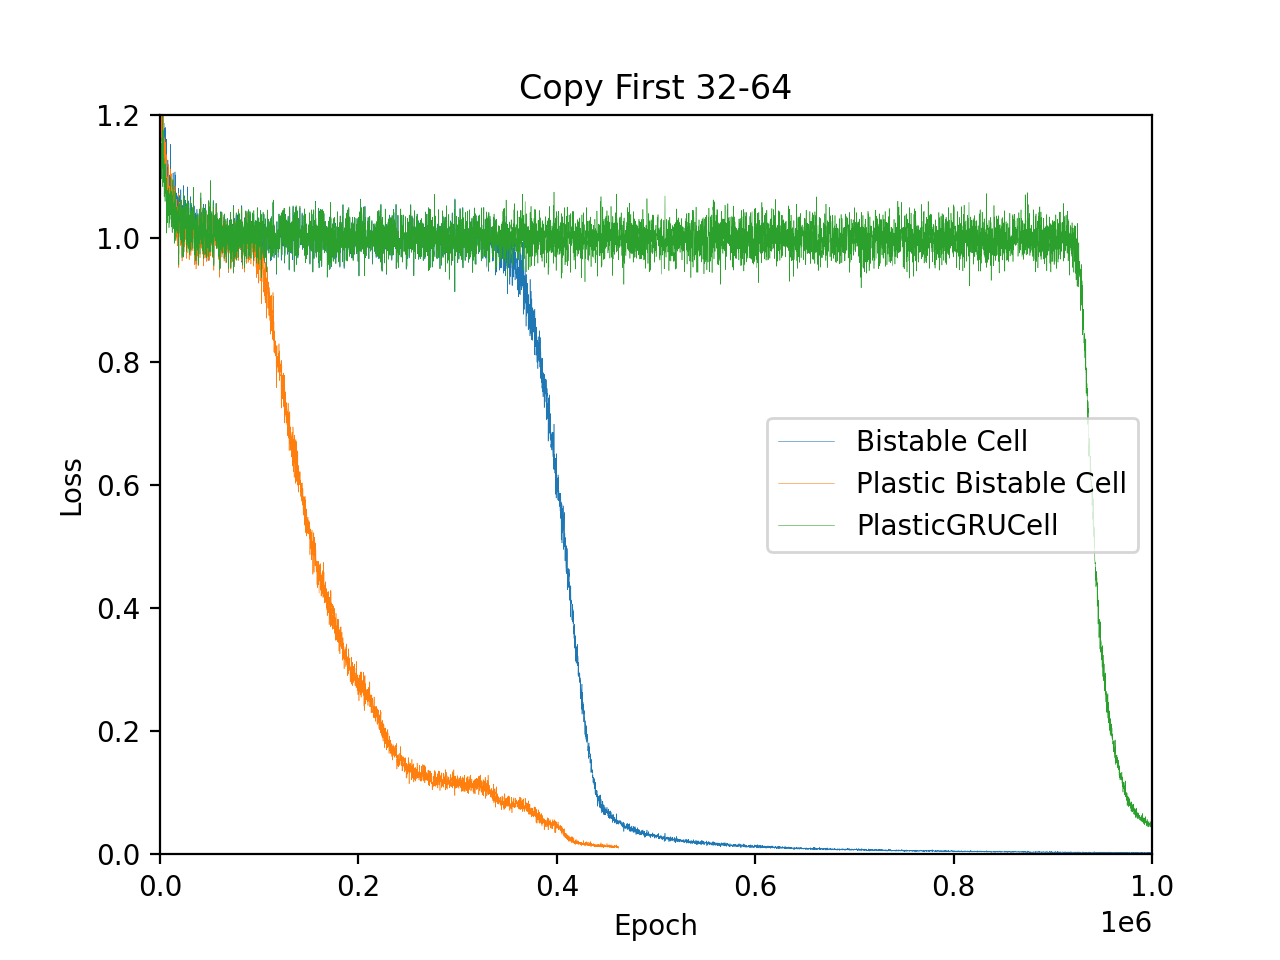
\includegraphics[width=6in]{plots/32_64_plot}
\end{figure}